\section{Existující řešení}
V rámci rešerše byly nalezeny čtyři aplikace. Konkrétně se jedná o aplikace \textit{sensor.community}, \textit{OpenAQ}, \textit{openSenseMap}, \textit{Indoor-CO2-Map}. Hloubkový výzkum ChatGPT našel aplikací celkem pět, ale poslední z nich, \textit{AirGradient},  se ukázala, že neměla být zahrnuta, protože se jedná pouze o prodejce hardwaru a ne o platformu pro sběr dat, která by byla relevantní pro tuto práci.

V první části této sekce je uveden stručný přehled každé z těchto aplikací a jejich funkcionalit. 
V druhé části jsou jednotlivé aplikace mezi sebou srovnány z pohledu funkcionalit webového rozhraní, licencí, sbíraných dat, sdílených dat pomicí API a pravidelných archivů (dumpů). Aplikace jsou také srovnány z pohledu otevřených formálních norem.

\subsection{Přehled aplikací}

\subsubsection{Aplikace sensor.community}

První aplikací je německá aplikace \textit{sensor.community} ze Stuttgartu. Aplikace je založena na komunitě dobrovolníků, kteří instalují senzory pro měření různých veličin a sdílejí je ve veřejné databázi. \parencite{SensorCommunityBuildYour}

Zaměření aplikace je především na měření kvality vnějšího prostředá, ale má možnost měřit i prostředí vnitřní.  

Ze zledovaných veličin uvedených v tabulce č. \ref{tab:sensor-community-veliciny} je zřejmé, že aplikace se zaměřuje především na sledování kvality vzduchu a to zejména z pohledu mikročástic PM a CO\textsubscript{2}, akustického komfortu a tepelného komfortu. Světelný komfort není v API/CSV exportech zastoupen.

\begin{table}[!tbp]
  \centering
  \footnotesize
  \setlength{\tabcolsep}{2pt}
  \renewcommand{\arraystretch}{1.1}
  \caption{Sledované veličiny aplikací sensor.community}
  \label{tab:sensor-community-veliciny}
  \begin{tabular}{p{2.8cm} p{5.8cm} p{1.7cm} >{\raggedright\arraybackslash}p{4.6cm}}
    \toprule
    \textbf{Kategorie} & \textbf{Veličina} & \textbf{Jednotka} & \textbf{Poznámka}\\
    \midrule
    \multirow{12}{*}{IAQ} & PM$_{1.0}$ (hmotnostní koncentrace) & $\mu$g/m$^3$ & ---\\
     & PM$_{2.5}$ (hmotnostní koncentrace) & $\mu$g/m$^3$ & ---\\
     & PM$_{4.0}$ (hmotnostní koncentrace) & $\mu$g/m$^3$ & Pouze některé senzory (např. SPS30, SEN5x).\\
     & PM$_{10}$ (hmotnostní koncentrace) & $\mu$g/m$^3$ & ---\\
     & Početní koncentrace částic $\geq$ 0.5\,$\mu$m & cm$^{-3}$ & \multirow{5}{4.6cm}{Nestandardní pro IEQ; početní (nikoli hmotnostní) metrika.}\\
     & Početní koncentrace částic $\geq$ 1.0\,$\mu$m & cm$^{-3}$ & \\
     & Početní koncentrace částic $\geq$ 2.5\,$\mu$m & cm$^{-3}$ & \\
     & Početní koncentrace částic $\geq$ 4.0\,$\mu$m & cm$^{-3}$ & \\
     & Početní koncentrace částic $\geq$ 10\,$\mu$m & cm$^{-3}$ & \\
     & Typická velikost částic & $\mu$m & Nestandardní pro IEQ.\\
     & CO$_2$ (koncentrace) & ppm & ---\\
     & NO$_2$ (měsíční průměr) & $\mu$g/m$^3$ & Z webového rozhraní\\
    \midrule
    \multirow{5}{*}{Akustický komfort} & LAeq (A-vážená ekvivalentní hladina) & dB(A) & ---\\
     & Minimální hladina (A) & dB(A) & ---\\
     & Maximální hladina (A) & dB(A) & ---\\
     & LA01 (1\,\% percentil) & dB(A) & Nestandardní pro IEQ (percentil).\\
     & LA95 (95\,\% percentil) & dB(A) & Nestandardní pro IEQ (percentil).\\
    \midrule
    \multirow{4}{*}{Tepelný komfort} & Teplota vzduchu & $^\circ$C & ---\\
     & Relativní vlhkost & \% & ---\\
     & Atmosférický tlak & Pa & Doplňkové (meteo).\\
     & Tlak přepočtený na hladinu moře & Pa & Doplňkové (meteo).\\
    \midrule
    \multirow{1}{*}{Světelný komfort} & --- & --- & V API/CSV exportech se nevyskytují veličiny vizuálního komfortu (např. osvětlenost).\\
    \bottomrule
  \end{tabular}

  \footnotesize \textit{Zdroj:} \parencite{Index, APIs}
\end{table}

V rámci funkcionalit webového rozhraní aplikace nabízí zobrazení dat na světové mapě. Uživatelé mohou zobrazení výsledků filtrovat podle (viz č. 2 na obrázku č. \ref{obr:sensor-community-filter}):
\begin{itemize}
  \item sledované veličiny; a to:
    \begin{itemize}
      \item NO$_{2}$,
      \item sensory na referenčních stanicích,
      \item rel. vlhokost,
      \item teplota,
      \item tlak,
      \item hluk,
      \item AQI US\footnote{\textit{Přeloženo z angličtiny pomocí DeepL: Index kvality ovzduší (AQI) se používá k informování o denní kvalitě ovzduší. Uvádí, jak čistý nebo znečištěný je vzduch ve vašem okolí a jaké související zdravotní dopady by pro vás mohly být důvodem k obavám. AQI se zaměřuje na zdravotní dopady, které se u vás mohou projevit během několika hodin nebo dnů po vdechnutí znečištěného vzduchu. EPA vypočítává AQI pro pět hlavních látek znečišťujících ovzduší, které jsou regulovány zákonem o čistém ovzduší: přízemní ozon, znečištění částicemi (známé také jako částicová hmota), oxid uhelnatý, oxid siřičitý a oxid dusičitý. Pro každou z těchto látek stanovila EPA národní normy kvality ovzduší s cílem chránit veřejné zdraví. Přízemní ozon a částice v ovzduší jsou dvě látky, které představují největší hrozbu pro lidské zdraví v této zemi.} \parencite{usdepartmentofcommerceAirQualityIndex}},
      \item PM$_{2.5}$,
      \item PM$_{10}$,
    \end{itemize}
  \item místní laboratoře,
  \item větrné vrstvy,
  \item Sensor2School,
  \item vnitřních senzorů.
\end{itemize}

Na rozhraní můžeme také vidět barevnou škálu pro právě vybranou veličinu (viz č. 1 na obrázku č. \ref{obr:sensor-community-filter}). Po vybrání veličiny je možné vybrat jeden či více zobrazovaných senzorů a získat tak konkrétní naměřenou hodnotu (viz obrázke č. \ref{obr:sensor-community-sensor-reading}). 

\begin{figure}[htbp!]\centering
\caption{Filtry a barevná škála pro zobrazení dat na mapě v aplikaci \textit{sensor.community}}
\label{obr:sensor-community-filter}
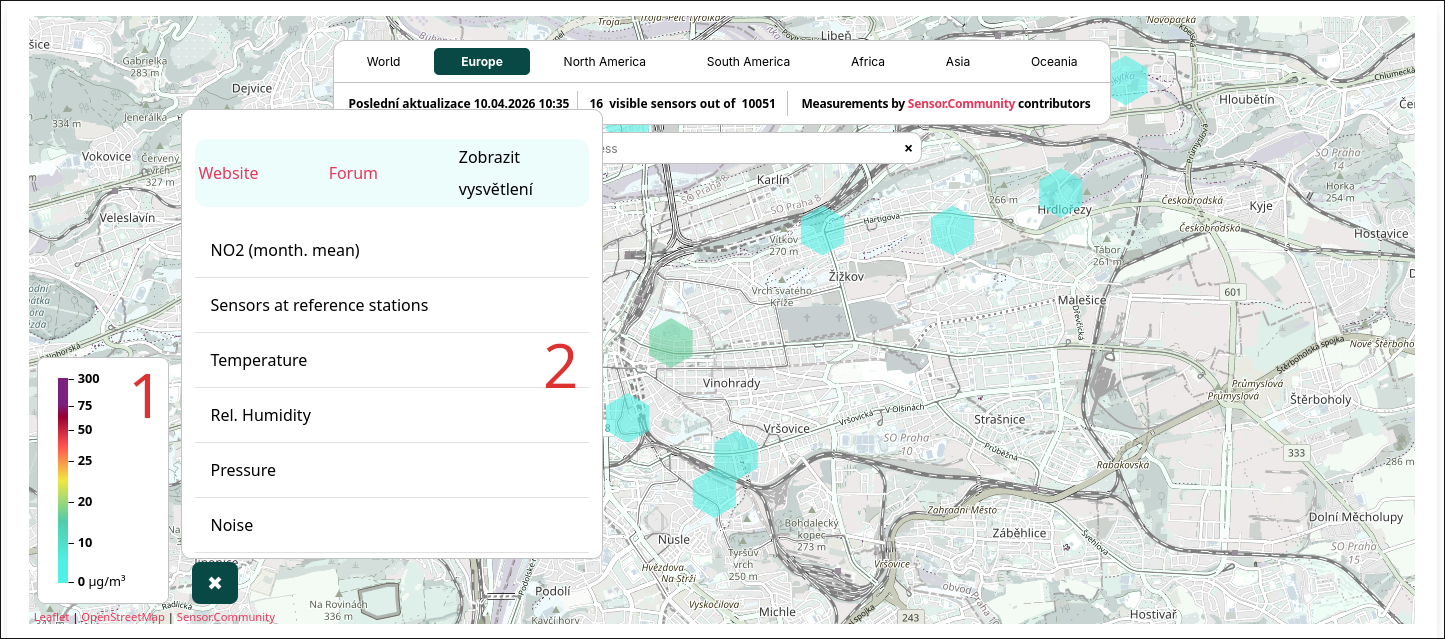
\includegraphics[width=.90\textwidth]{img/sensor-community-filtry}

\footnotesize \textit{Poznámka: 1 - barevná škála, 2 - filtry pro zobrazení dat na mapě.}

\footnotesize \textit{Zdroj:} Pořízeno autorem z webového rozhraní aplikace. 
\end{figure}

\begin{figure}[htbp!]\centering
\caption{Konkrétní senzor na mapě a jeho hodnota na webu \textit{sensor.community}}
\label{obr:sensor-community-sensor-reading}
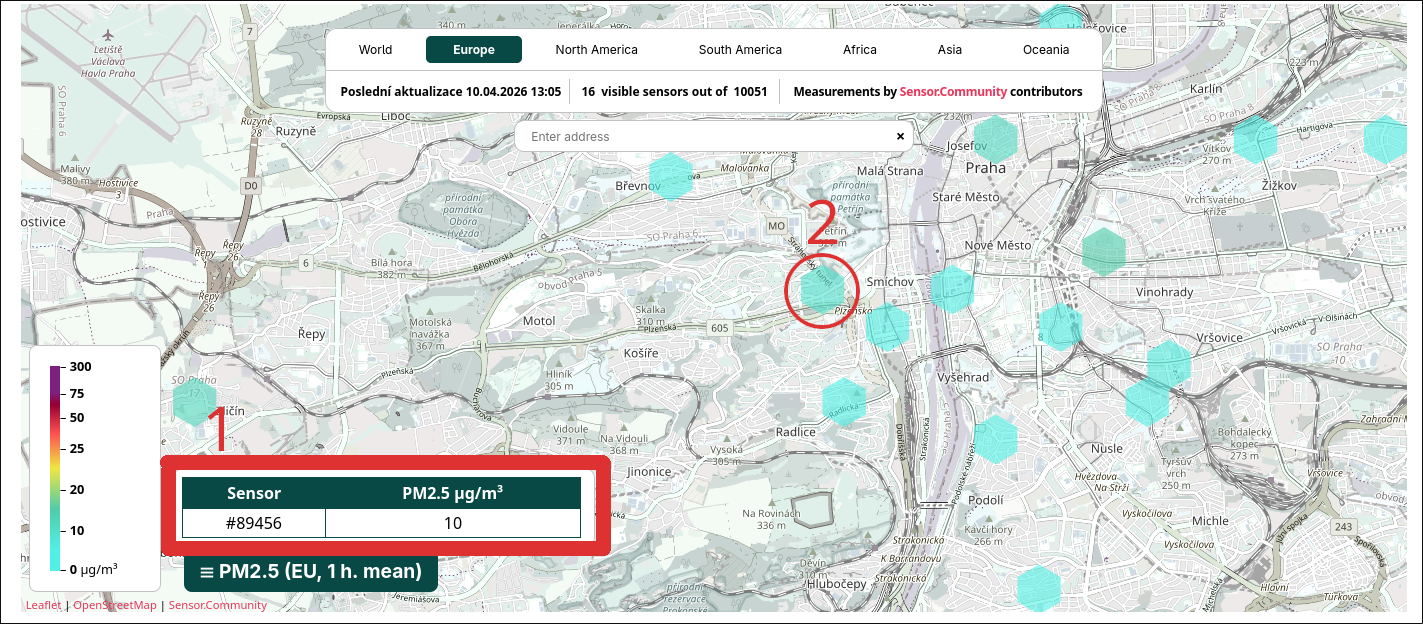
\includegraphics[width=.90\textwidth]{img/sensor-community-mapa-body}

\footnotesize \textit{Poznámka: 1 - konkrétní hodnota změřená vybraným senzorem, 2 - Klikatelný senzor na mapě. }

\footnotesize \textit{Zdroj:} Pořízeno autorem z webového rozhraní aplikace. 
\end{figure}

V tabulce č. \ref{tab:sensor-community-supported-sensors} je uveden přehled podporovaných senzorů aplikací Sensor.Community a veličin, které měří. V tabulce jsou uvedeny pouze veličiny, které jsou relevantní pro IEQ. Je nutné poznamenat, že aplikace v rámci některých senzorů nesbírá veškeré veličiny, které je daný senzor schopen měřit. Například u v rodině senzorů SEN5x existují senzory schopné měřit TVOC, ale v aplikaci, ať už v API, v CSV exportech nebo na webovém rozhraní, se veličina TVOC nevyskytuje. 

\clearpage
{
  \footnotesize
  \setlength{\tabcolsep}{2pt}
  \renewcommand{\arraystretch}{1.1}
  \begin{longtable}{*{1}{l}@{\hspace{12pt}}*{8}{c}@{\hspace{12pt}}*{3}{c}@{\hspace{12pt}}*{2}{c}@{\hspace{12pt}}*{2}{c}}
    \caption{Podporovné senzory sensor.community a jejich měřené veličiny}
    \label{tab:sensor-community-supported-sensors}\\
    \toprule
    \multirow{3}{*}{\textbf{Senzor}} & \multicolumn{15}{c}{\textbf{Kategorie IEQ}} \\
                                     & \multicolumn{8}{c}{\textbf{IAQ}} & \multicolumn{3}{c}{\textbf{TK}} & \multicolumn{2}{c}{\textbf{SK}} & \multicolumn{2}{c}{\textbf{AK}} \\
                                     & PM\textsubscript{2.5} & PM\textsubscript{10} & O\textsubscript{3} & NO\textsubscript{2} & SO\textsubscript{2} & CO & CO\textsubscript{2} & TVOC & $T$ & RH & $v$ & $E$ & CCT & $L_A$ & $L$ \\
                                     \hline
BME280 &  &  &  &  &  &  &  &  & \cmark & \cmark &  &  &  &  &  \\ % T, RH, P
\hline
BMP180 &  &  &  &  &  &  &  &  & \cmark &  &  &  &  &  &  \\ % T, P
\hline
BMP280 &  &  &  &  &  &  &  &  & \cmark &  &  &  &  &  &  \\ % T, P
\hline
DHT22 &  &  &  &  &  &  &  &  & \cmark & \cmark &  &  &  &  &  \\ % T, RH
\hline
DS18B20 & & & & & & & & & \cmark & & & & & &  \\ % T
\hline
DS18S20 & & & & & & & & & \cmark & & & & & & \\ % T
\hline
GPS-NEO-6M & & & & & & & & & & & & & & & \\ % GPS
\hline
HM3301 & \cmark & \cmark & & & & & & & & & & & & & \\ % PM1.0, PM2.5, PM10
\hline
HPM & \cmark & \cmark & & & & & & & & & & & & & \\ % PM2.5, PM10 output (standard); PM1.0, PM2.5, PM4.0
\hline
HTU21D & & & & & & & & & \cmark & \cmark & & & & & \\ % T, RH
\hline
IPS-7100 & \cmark & \cmark & & & & & & & & & & & & & \\ %PM (all)
\hline
DNMS (Laerm) & & & & & & & & & & & & & & \cmark & \\ % Noise
\hline
NextPM & \cmark & \cmark & & & & & & & & & & & & & \\ % PM2.5, PM10
\hline
NO2-A43F & & & & \cmark & & & & & & & & & & & \\ %NO2
\hline
PMS1003 & \cmark & & & & & & & & & & & & & & \\ %PM2.5, mozna PM10
\hline
PMS3003 & \cmark & & & & & & & & & & & & & & \\ %PM2.5
\hline
PMS5003 & \cmark & \cmark & & & & & & & & & & & & & \\ % PM1.0 PM2.5, PM10
\hline
PMS6003 & \cmark & & & & & & & & & & & & & & \\ %PM2.5
\hline
PMS7003 & \cmark & & & & & & & & & & & & & & \\ %PM2.5
\hline
PPD42NS & \cmark & & & & & & & & & & & & & & \\ %PM2.5, dust
\hline
Radiation SBM-19 & & & & & & & & & & & & & & & \\ %radiation
\hline
Radiation SBM-20 & & & & & & & & & & & & & & & \\ %radiation
\hline
Radiation Si22G & & & & & & & & & & & & & & & \\ %radiation
\hline
SCD30 & & & & & & & \cmark & & \cmark & \cmark & & & & & \\
\hline
SDS011 & \cmark & \cmark & & & & & & & & & & & & & \\
\hline
SDS021 & \cmark & \cmark & & & & & & & & & & & & & \\
\hline
SEN5x & \cmark & \cmark & & \cmark & & & & \cmark & \cmark & \cmark & & & & & \\
\hline
SHT10 & & & & & & & & & \cmark & \cmark & & & & & \\
\hline
SHT11 & & & & & & & & & \cmark & \cmark & & & & & \\
\hline
SHT15 & & & & & & & & & \cmark & \cmark & & & & & \\
\hline
SHT30 & & & & & & & & & \cmark & \cmark & & & & & \\
\hline
SHT31 & & & & & & & & & \cmark & \cmark & & & & & \\
\hline
SHT35 & & & & & & & & & \cmark & \cmark & & & & & \\
\hline
SHT85 & & & & & & & & & \cmark & \cmark & & & & & \\
\hline
SPS30 & \cmark & \cmark & & & & & & & & & & & & & \\
    \bottomrule
  \end{longtable}

  \footnotesize \textit{Zdroj: }Vlastní zpracování, \parencite{APISensorCommunity, SensorCommunityDevices}

  \footnotesize \textit{Poznámka:} Senzory \textit{Radiation SBM-19}, \textit{Radiation SBM-20} a \textit{Radiation Si22G} jsou určeny pro měření radiace, což autorem nebylo identifikováno jako měřená veličina relevantní pro IEQ. To samé se dá říci i o senzoru \textit{GPS-NEO-6M}, který je modulem GPS a má význam pouze pro lokalizaci senzoru.
}
\clearpage



\subsubsection{Aplikace OpenAQ}

\[DRAFT\]

Druhou aplikací je americká aplikace \textit{OpenAQ} z New Yorku. Tato aplikace se, jak je uvedeno v dokumentaci API, zaměřuje především na měření kvality vnějšiho ovzduší. Podporovné veličiny jsou uvedeny v tabulce č. \ref{tab:open-aq-veliciny} \parencite{API}. Z té je zřejmé, že aplikace vůbec nemyslí na měření veličin akustického či světelného komfortu. 

Data v aplikaci OpenAQ jsou poskytována dvěma způsoby. 
Prvním z nich je přístup přes REST API, který umožňuje získat data ve formátu JSON. Tento přistup je vhodné pro programatické zpracování dat. Pro používání API jsou dostupné sady vývojových nástrojů (SDK) pro skriptovací jazyky Python a R. \parencite{API}  

Druhým způsobem je pravidelný archiv dat, který je dostupný na platformě AWS v S3 bucketu. Data jsou zde sdílena měsíčně ve formátu komprimovaných CSV souborů pomocí gzip. \parencite{zotero-item-552}

\begin{table}[!tbp]
  \centering
  \footnotesize
  \setlength{\tabcolsep}{2pt}
  \renewcommand{\arraystretch}{1.1}
  \caption{Sledované veličiny aplikací OpenAQ}
  \label{tab:open-aq-veliciny}
  \begin{tabular}{lllL{4cm}}
    \toprule
    \textbf{Kategorie} & \textbf{Veličina} & \textbf{Jednotka} & \textbf{Poznámka}\\
    \midrule
    \multirow{14}{*}{IAQ} 
                       & PM$_{1.0}$ & $\mu$g/m$^3$, cm$^{-3}$ & ---\\
                       & PM$_{2.5}$ & $\mu$g/m$^3$, ppm, cm$^{-3}$ & ---\\
     & PM$_{4.0}$ & $\mu$g/m$^3$ & ---\\
     & PM$_{10}$ & $\mu$g/m$^3$, cm$^{-3}$ & ---\\
     & CO & $\mu$g/m$^3$, ppm, ppb & ---\\
     & CO$_2$ & ppm & ---\\
     & NO & $\mu$g/m$^3$, ppm, ppb & ---\\
     & NO$_2$ & $\mu$g/m$^3$, ppm, ppb & ---\\
     & NO$_x$ & $\mu$g/m$^3$, ppm, ppb & ---\\
     & SO$_2$ & $\mu$g/m$^3$, ppm, ppb & ---\\
     & O$_3$ & $\mu$g/m$^3$, ppm, ppb & ---\\
     & BC & $\mu$g/m$^3$, ng/m$^3$ & Black Carbon (BC) - částice uhlíku menší než PM$_{2.5}$.\\ 
     & CH$_4$ & ppm & Metan. \\ 
     & UFP & cm$^{-3}$ & Ultra Fine Particles (UFP), někdy označována jako PM$_{0.1}$ jsou částice o velikostech v řádu desítek nanometrů.\\ 
     & P & hPa, mb & ---\\
    \midrule
    \multirow{1}{*}{Akustický komfort} & --- & --- & ---\\
    \midrule
    \multirow{2}{*}{Tepelný komfort} & $T$ & $^\circ$C, $^\circ$F & ---\\
     & RH & \% & ---\\
     & $v$ & m/s & ---\\
    \midrule
    \multirow{1}{*}{Světelný komfort} & --- & --- & --- \\
    \bottomrule
  \end{tabular}

  \footnotesize \textit{Zdroj:} Vlastní zpracování na základě dat z \parencite{API, zotero-item-549, UltrajemneCastice2025, CernyUhlik2025}. 
\end{table}

Za pomocí API byly identifikovány senzory, které jsou na plarformě OpenAQ použávány. Jejich shrnutí je uvedeno v tabulce č. \ref{tab04:openaq-supported-sensors}. V tabulce jsou uvedeny pouze veličiny, které jsou relevantní pro IEQ a byly v rámci rešerše autorem identifikovány. Je nutné poznamenat, že aplikace není závislá na konkrétním hardwaru. Uvedené senzory jsou pouze příklady, kdy autoři dat publikovali, jaký konkrétní hardware používají. To umožňuje uživatelům dat lépe porozumět, s jakou spolehlivostí a přesností data interpretovat. \parencite{API}

Praxe, kdy aplikace není závislá na konkrétním hardwaru je výhodná z pohledu udržitelnosti aplikace, kdy není potřeba implementovat podporu pro každý nový senzor. Tímto způsobem je břemeno napojení přeneseno na uživatele, který se rozhodne data publikovat. Tím se může vstupní bariéra pro publikování dat zvýšit, ale zároveň se zvyšuje flexibilita a škálovatelnost platformy.

{
  \footnotesize
  \setlength{\tabcolsep}{2pt}
  \renewcommand{\arraystretch}{1.1}
  \begin{longtable}{L{3.3cm}@{\hspace{8pt}}*{8}{c}@{\hspace{8pt}}*{3}{c}@{\hspace{8pt}}*{2}{c}@{\hspace{8pt}}*{2}{c}}
    \caption{Podporované instrumenty OpenAQ a jejich měřené veličiny relevantní pro IEQ}
    \label{tab04:openaq-supported-sensors}\\
    \toprule
    \multirow{3}{*}{\textbf{Senzor}} & \multicolumn{15}{c}{\textbf{Kategorie IEQ}} \\
                                     & \multicolumn{8}{c}{\textbf{IAQ}} & \multicolumn{3}{c}{\textbf{TK}} & \multicolumn{2}{c}{\textbf{SK}} & \multicolumn{2}{c}{\textbf{AK}} \\
                                     & PM\textsubscript{2.5} & PM\textsubscript{10} & O\textsubscript{3} & NO\textsubscript{2} & SO\textsubscript{2} & CO & CO\textsubscript{2} & TVOC & $T$ & RH & $v$ & $E$ & CCT & $L_A$ & $L$ \\
                                     \hline
Government Monitor & \cmark & \cmark & \cmark & \cmark & \cmark & \cmark & & & & & & & & & \\
\hline
Clarity Node-S (Clarity Sensor) & \cmark & & & \cmark & & & & & & & & & & & \\
\hline
HabitatMap AirBeam (HabitatMap Sensor) & \cmark & & & & & & & & & & & & & & \\
\hline
Senstate Sensor & & & & & & & & & & & & & & & \\
\hline
BEACO2N Sensor & \cmark & & & \cmark & & & \cmark & & \cmark & \cmark & & & & & \\
\hline
RAMP Sensor & & & \cmark & \cmark & \cmark & \cmark & & & & & & & & & \\
\hline
Aerosol Black Carbon Detector (ABCD) & & & & & & & & & & & & & & & \\
\hline
MA350 (AethLabs) & & & & & & & & & & & & & & & \\
\hline
Met One AIO 2 & \cmark & \cmark & & & & & & & & & & & & & \\
\hline
Met One BAM 1020 & \cmark & \cmark & & & & & & & & & & & & & \\
\hline
Met One BAM 1022 & \cmark & \cmark & & & & & & & & & & & & & \\
\hline
Serinus 30 (Ecotech) & & & & & & \cmark & & & & & & & & & \\
\hline
AirVisual (IQAir) & \cmark & & & & & & & & & & & & & & \\
\hline
AirGradient ONE (8PSL) & \cmark & \cmark & & & & & \cmark & \cmark & \cmark & \cmark & & & & & \\
\hline
AirGradient ONE (8PSL-DE) & \cmark & \cmark & & & & & \cmark & \cmark & \cmark & \cmark & & & & & \\
\hline
AirGradient ONE Gen 9 (I-9PSL) & \cmark & \cmark & & & & & \cmark & \cmark & \cmark & \cmark & & & & & \\
\hline
AirGradient ONE Gen 9 (I-9PSL-DE) & \cmark & \cmark & & & & & \cmark & \cmark & \cmark & \cmark & & & & & \\
\hline
AirGradient Open Air (O-1PST-CE) & \cmark & \cmark & & & & & & & \cmark & \cmark & & & & & \\
\hline
AirGradient Open Air Gen 1 (O-1PST) & \cmark & \cmark & & & & & & & \cmark & \cmark & & & & & \\
\hline
AirGradient Open Air (O-1PPT-CE) & \cmark & \cmark & & & & & & & \cmark & \cmark & & & & & \\
\hline
AirGradient Open Air Max Gen 1 (O-M-1PPST-CE) & \cmark & \cmark & & & & & & & \cmark & \cmark & & & & & \\
\hline
AirGradient Open Air Max Gen 1 (O-M-1PPSTON-CE) & \cmark & \cmark & & \cmark & & & & & \cmark & \cmark & & & & & \\
\hline
AirGradient DIY-Basic Gen 1-3 (I-1DIY) & \cmark & \cmark & & & & & \cmark & \cmark & \cmark & \cmark & & & & & \\
\hline
Aernode (Quanta S.r.l.) & \cmark & \cmark & \cmark & \cmark & \cmark & \cmark & & & \cmark & \cmark & & & & & \\
\hline
Miri Air (Miri Africa) & \cmark & \cmark & & & & & \cmark & & \cmark & \cmark & & & & & \\
    \bottomrule
  \end{longtable}

  \footnotesize \textit{Zdroj: }Vlastní zpracování za pomocí umělé inteligence na základě dat \parencite{API} a veřejně dostupných technických podkladů výrobců.

  \footnotesize \textit{Poznámka:} Seznam instrumentů OpenAQ obsahuje 27 položek. V tabulce jsou uvedeny jednotlivé instrumenty (bez slučování do rodin). Položky \textit{N/A} a \textit{Unknown AirGradient Sensor} nejsou uvedeny, protože nejde o konkrétní dohledatelná zařízení. Veličiny Black Carbon (např. \textit{MA350}, \textit{ABCD}) nejsou vyznačeny, protože nejsou samostatným sloupcem v použité IEQ matici.
}

Webové rozhraní aplikace je pro zobrazování dat na světové mapě podobné jako u aplikace Sensor.Community. Uživatelské rozrhraní je pro zobrazování dat přístupné bez předchozí regitrace. Uživatelé mohou zobrazení výsledků filtrovat podle: 
\begin{itemize}
  \item sledované znečisťující látky; a to:
    \begin{itemize}
      \item jakékoliv znečišťující látky (bez omezení),
      \item PM$_{2.5}$,
      \item PM$_{10}$,
      \item O$_{3}$,
      \item NO$_{2}$,
      \item SO$_{2}$,
      \item CO,
    \end{itemize}
  \item typu sledované lokality; těmi jsou:
    \begin{itemize}
      \item referenční stanice,
      \item lokace senzoru vzduchu,
      \item lokace senzoru, který nevykazuje aktivity,
    \end{itemize}
  \item dle partnerských projektů,
  \item a dle poskytovatele dat (171 poskytovatelů v době zpracování této části).
\end{itemize}

Tyto filtry jsou zobrazeny na obrázku č. 



\subsubsection{Aplikace openSenseMap}

Třetí analyzovanou aplikací je německá aplikace \textit{openSenseMap}, která je vyvíjena v rámci projektu \textit{senseBox} na Univerzitě v Münsteru. Aplikace slouží jako platforma pro sběr, vizualizaci a sdílení environmentálních dat pocházejících z občanských vědeckých projektů a individuálních senzorových stanic. \parencite{SenseboxOpenSenseMap2026} Primárním zaměřením je monitorování vnějšího prostředí, platforma však umožňuje rozlišovat mezi senzory umístěnými ve venkovním prostředí (\textit{outdoor}), vnitřním prostředí (\textit{indoor}) a mobilními senzory (\textit{mobile}). Tato klasifikace umožňuje uživatelům dat filtrovat a analyzovat pouze data relevantní pro konkrétní typ prostředí. \parencite{OpenSenseMapAPIDocumentation}

Data z platformy openSenseMap jsou přístupná třemi způsoby. Prvním je \textit{REST API}, které poskytuje data ve formátech JSON, GeoJSON a CSV. API umožňuje dotazování na metadata senzorových stanic, jednotlivá měření i hromadný export dat z více stanic současně. Dotazy lze filtrovat podle sledované veličiny, geografické oblasti, typu prostředí nebo modelu senzorové stanice. Pro jednotlivý senzor je omezení na 10\,000 záznamů, resp. maximálně 1 měsíc dat na jeden dotaz. Pro čtení dat není vyžadována autentizace; ta je nutná pouze pro operace zápisu. \parencite{OpenSenseMapAPIDocumentation}

Druhým způsobem přístupu je \textit{archiv dat}, dostupný na adrese \href{https://archive.opensensemap.org/}{archive.opensensemap.org}. Archiv obsahuje denní exporty měření ve formátu CSV a metadata senzorových stanic ve formátu JSON. Data v archivu jsou organizována do adresářů podle dnů a jednotlivých senzorových stanic, přičemž záznamy jsou k dispozici od června 2014. Archiv je veřejně přístupný bez autentizace a je vhodný pro hromadné stahování historických dat. \parencite{zotero-item-562}

Třetím způsobem je \textit{webové rozhraní} na adrese \href{https://opensensemap.org/}{opensensemap.org}, které umožňuje prohlížení dat na interaktivní mapě (viz obrázek č.~\ref{obr:opensensemap-web}), filtrování podle veličin (viz obrázek č.~\ref{obr:opensensemap-filters}) a zobrazení grafů naměřených hodnot (viz obrázek č.~\ref{obr:opensensemap-sensor-reading}). Webové rozhraní je určeno především pro vizuální průzkum dat a neposkytuje možnost hromadného exportu dat; pro ten je nutné využít API nebo archiv. \parencite{SenseboxOpenSenseMap2026}

\begin{figure}[htbp!]\centering
\caption{Webové rozhraní aplikace openSenseMap}
\label{obr:opensensemap-web}
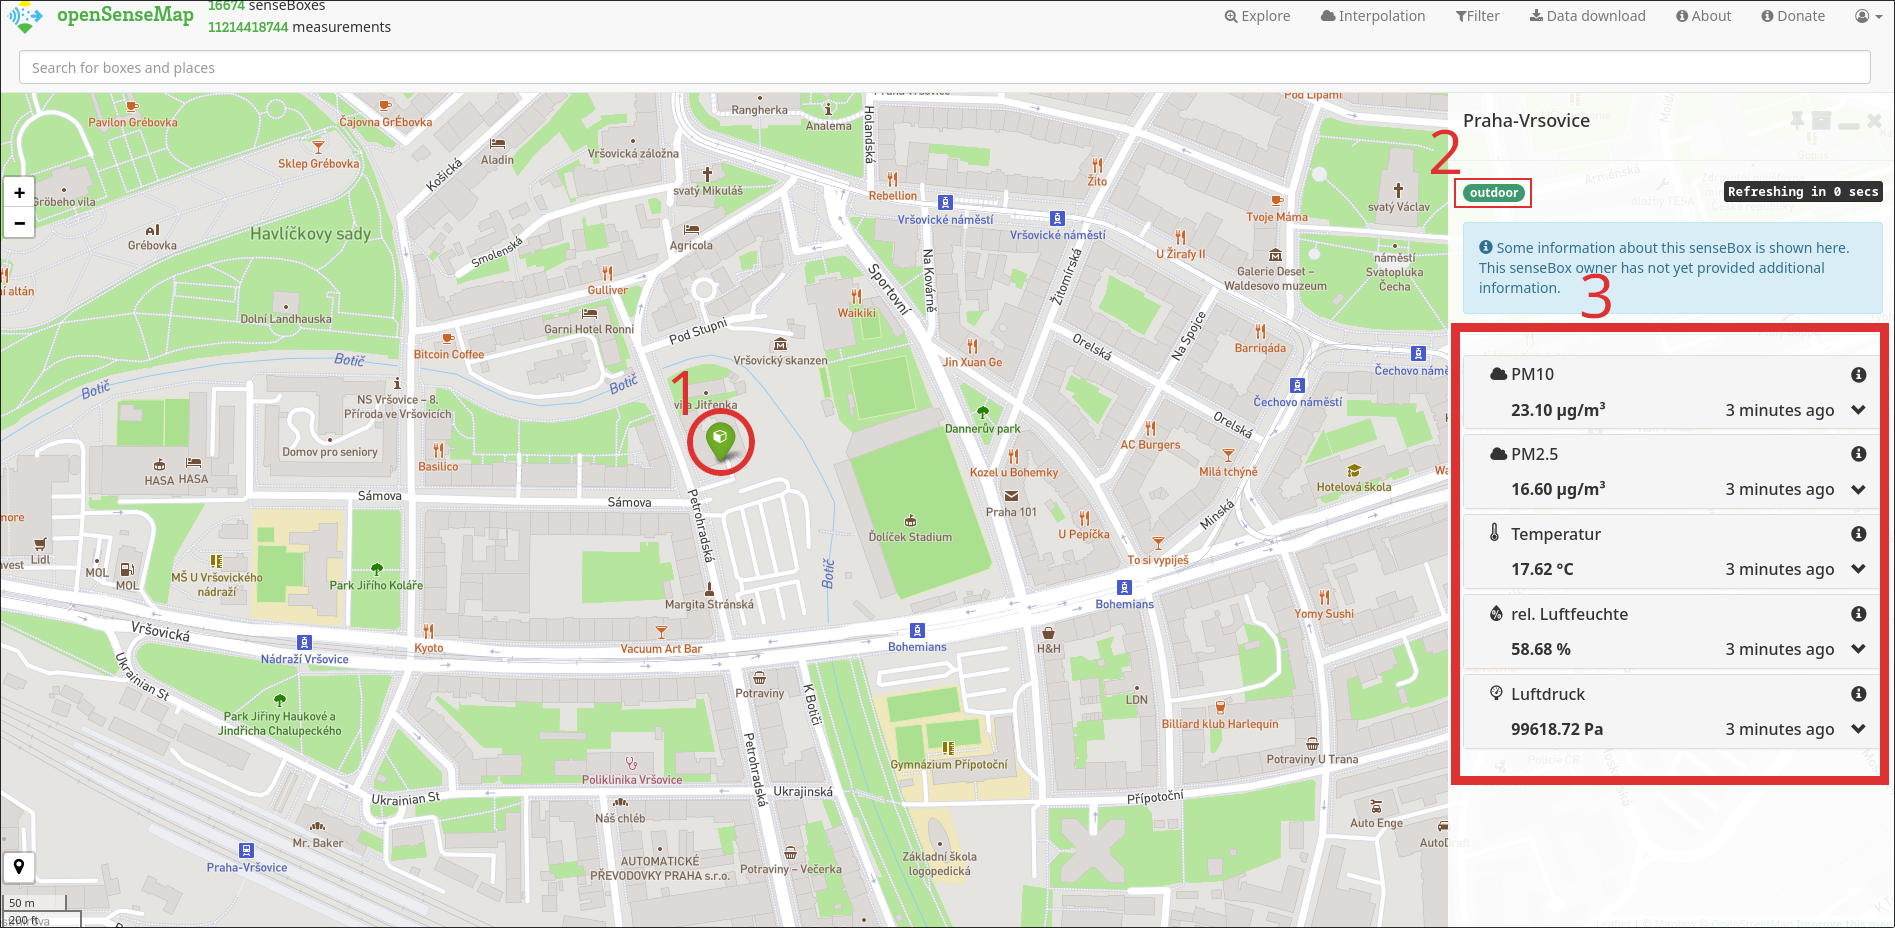
\includegraphics[width=.90\textwidth]{img/opensensemap-map}

\footnotesize \textit{Poznámka:} 1 - konkrétní senzorová stanice zobrazená na mapě, 2 - umístění senzoru (indoor, outdoor, mobile), 3 - měřené veličiny a aktuálně naměřené hodnoty

\footnotesize \textit{Zdroj:} Snímek obrazovky pořízen autorem z webového rozhraní aplikace.
\end{figure}

\begin{figure}[htbp!]\centering
\caption{Bodový graf vybrané měřené veličiny konkrétního senzoru v aplikaci openSenseMap}
\label{obr:opensensemap-sensor-reading}
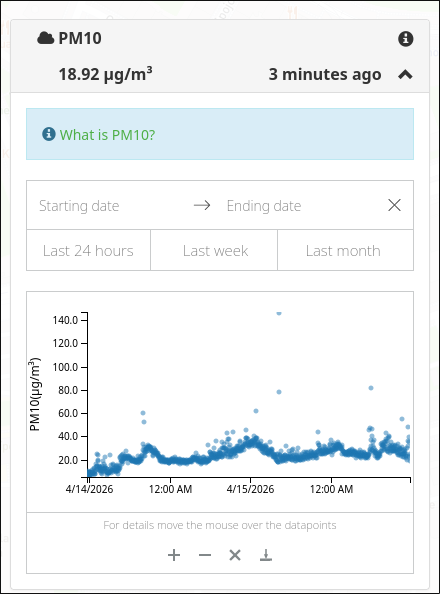
\includegraphics[width=.90\textwidth]{img/opensensemap-reading}

\footnotesize \textit{Poznámka:} Ukázka bodovégo grafu zobrazujícího jednotlivé naměřené hodnoty vybrané veličiny za vybrané časové období pro konkrétní senzor. 

\footnotesize \textit{Zdroj:} Snímek obrazovky pořízen autorem z webového rozhraní aplikace.
\end{figure}

\begin{figure}[htbp!]\centering
\caption{Filtry zobrazení webového rozhraní v aplikaci openSenseMap}
\label{obr:opensensemap-filters}
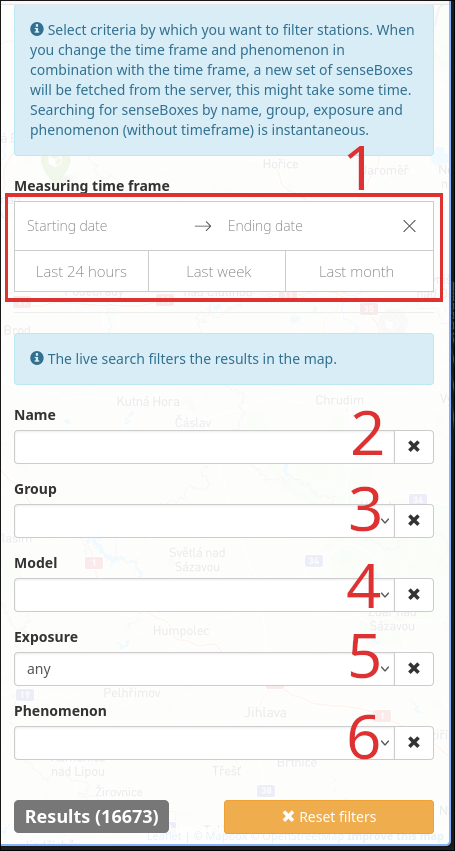
\includegraphics[width=.70\textwidth]{img/opensensemap-filters}

\footnotesize \textit{Poznámka:} 1 - omezení časového období, 2 - omezení dle jména, 3 - omezení dle skupiny, do které uživatel senzor zařadil, 4 - omezení dle modelu (senseBox, Luftdaten, vlastní), 5 - omezení dle typu prostředí (indoor, outdoor, mobile), 6 - omezení dle sledované veličiny

\footnotesize \textit{Zdroj:} Snímek obrazovky pořízen autorem z webového rozhraní aplikace.
\end{figure}


Na rozdíl od aplikací Sensor.Community a OpenAQ nemá platforma openSenseMap pevně daný výčet sledovaných veličin ani předem definovaný seznam podporovaných senzorů. Při registraci senzorové stanice uživatel volně definuje název veličiny, měrnou jednotku a typ senzoru jako textové řetězce. Platforma tak může přijímat data z libovolného senzoru, který uživatel připojí. Pro usnadnění registrace nabízí platforma předdefinované šablony senzorových stanic (např. \textit{senseBox:home} v různých verzích), které obsahují běžné kombinace senzorů pro měření teploty, vlhkosti, atmosférického tlaku, osvětlenosti, UV záření, koncentrace mikročástic PM\textsubscript{2,5} a PM\textsubscript{10}, VOC, CO\textsubscript{2} a hladiny hluku. Tyto šablony jsou však pouze doporučením a uživatel je může libovolně upravit. \parencite{SenseboxOpenSenseMapAPI2026}

Tato otevřenost přináší významnou výhodu ve flexibilitě, neboť platforma není vázána na konkrétní hardware a nevyžaduje aktualizaci při uvedení nového typu senzoru na trh. Zároveň však přináší problémy spojené s konzistencí dat. Stejná fyzikální veličina může být na platformě evidována pod různými názvy (např. \textit{Temperatur}, \textit{Lufttemperatur}, \textit{Temperature}), v různých jednotkách a s různými typy senzorů. Tento stav ztěžuje agregaci a srovnávání dat napříč senzory a vyžaduje od uživatelů dat dodatečnou normalizaci. \parencite{SenseboxOpenSenseMapAPI2026}

Z hlediska veličin relevantních pro IEQ platforma prostřednictvím předdefinovaných šablon podporuje měření teploty vzduchu, relativní vlhkosti, atmosférického tlaku, koncentrace mikročástic (PM\textsubscript{1}, PM\textsubscript{2,5}, PM\textsubscript{4}, PM\textsubscript{10}), VOC (jako odpor senzoru v k$\Omega$), CO\textsubscript{2} (v ppm), osvětlenosti (v lx), UV intenzity (v $\mu$W/cm$^2$), hladiny hluku (v dB(A)) a rychlosti větru. Plynné polutanty jako O\textsubscript{3}, NO\textsubscript{2}, SO\textsubscript{2} a CO nejsou součástí předdefinovaných šablon a v datech platformy se vyskytují pouze ojediněle v rámci uživatelsky definovaných senzorů. \parencite{SenseboxOpenSenseMapAPI2026, OpenSenseMapAPIDocumentation}


\subsubsection{Aplikace IndoorCO2Map}

Čtvrtou analyzovanou aplikací je německá aplikace \textit{IndoorCO2Map}, jejímž autorem je Aurel Wünsch z Lipska. Na rozdíl od ostatních analyzovaných aplikací, které se zaměřují primárně na monitorování vnějšího prostředí, je \textit{IndoorCO2Map} orientována výhradně na vnitřní prostředí veřejně přístupných budov, jako jsou obchody, restaurace, školy, nemocnice či prostředky veřejné dopravy. Projekt se skládá z mobilní aplikace pro sběr dat (Android a iOS) a webového rozhraní pro jejich vizualizaci. Měřenou veličinou je výhradně koncentrace CO\textsubscript{2} v jednotkách ppm. \parencite{IndoorCO2MapCO2Monitoring2024}

Zdrojový kód mobilní aplikace je k dispozici ve dvou verzích: starší V1 pod licencí MIT \parencite{aurelwuAurelWuIndoorCO2AppMAUI2026} a novější V2 pod licencí GPLv2 \parencite{aurelwuAurelWuIndoorCO2MapApp2026}. Nasbíraná data jsou publikována pod licencí CC0 1.0 Universal (Public Domain), což umožňuje jejich volné využití bez jakýchkoli omezení \parencite{zotero-item-571}.

Na rozdíl od ostatních aplikací, u nichž je přehled sledovaných veličin shrnut v samostatné tabulce, u aplikace \textit{IndoorCO2Map} není tabulka veličin účelná, neboť aplikace měří výhradně koncentraci CO\textsubscript{2}. Žádné další veličiny relevantní pro IEQ (teplota, relativní vlhkost, koncentrace mikročástic, hladina hluku, osvětlenost apod.) nejsou sbírány ani přenášeny na backend. Některé podporované senzory (např. Airvalent) sice hardwarově měří i teplotu, avšak aplikace tyto hodnoty neextrahuje \parencite{aurelwuAurelWuIndoorCO2MapApp2026}. Na webovém rozhraní je z naměřených hodnot CO\textsubscript{2} odvozováno tzv. GO IAQS skóre na stupnici 0--10, které slouží jako zjednodušený indikátor kvality vnitřního vzduchu \parencite{IndoorCO2Atlas}.

Data z aplikace \textit{IndoorCO2Map} jsou přístupná dvěma způsoby. Aplikace neposkytuje žádné veřejné REST ani jiné API pro čtení dat. Webové rozhraní nenačítá data z API, ale ze statického předgenerovaného JSON souboru. Existuje pouze interní API pro zápis dat z mobilní aplikace, které odesílá měření prostřednictvím HTTPS POST požadavků na cloudovou infrastrukturu Amazon Web Services (AWS) \parencite{aurelwuAurelWuIndoorCO2MapApp2026}.

Prvním způsobem přístupu k datům je \textit{archiv dat} ke stažení.\footnote{\url{https://indoorco2map.com/chartdata/IndoorCO2MapData.zip}} Je k dispozici ZIP archiv obsahující kompletní datovou sadu ve formátu JSON (19\,720 záznamů v~době stažení), soubor s licencí CC0 1.0 Universal a popis datových polí. Každý záznam obsahuje typ a identifikátor prvku z OpenStreetMap (OSM), název lokality, GPS souřadnice, kód země dle ISO 3166-1 alpha-3, NUTS\,3 region, OSM klíč a tag, začátek měření ve formátu ISO 8601, informace o otevřených oknech a ventilaci, pole hodnot CO\textsubscript{2} v~ppm, interval měření a průměrnou hodnotu CO\textsubscript{2} \parencite{zotero-item-571}.

Druhým způsobem je \textit{webové rozhraní} na adrese \href{https://indoorco2map.com}{indoorco2map.com}, které zobrazuje nasbíraná data na interaktivní mapě (viz obrázek č.~\ref{obr:indoorco2map-map}). Data jsou načítána z~předgenerovaného komprimovaného JSON souboru, nikoli z~API v~reálném čase. Jednotlivé body na mapě představují konkrétní místa měření a jsou barevně odlišeny podle dosaženého GO IAQS skóre. Po kliknutí na vybraný bod se zobrazí detail měření včetně grafu průběhu koncentrace CO\textsubscript{2} v~čase. Webové rozhraní disponuje sadou filtrů (viz obrázek č.~\ref{obr:indoorco2map-filters}), které umožňují omezit zobrazená data podle názvu lokality, země, typu lokality odvozeného z~OSM tagů (např. supermarket, škola, nemocnice), časového rozsahu a rozsahu GO IAQS skóre. Součástí panelu filtrů je histogram distribuce lokací podle průměrné koncentrace CO\textsubscript{2} v~aktuálně vyfiltrované oblasti (viz obrázek č.~\ref{obr:indoorco2map-filters-histogram}). Prostřednictvím navigačního menu (viz obrázek č.~\ref{obr:indoorco2map-menu}) má uživatel přístup k~dalším analytickým pohledům, jako jsou souhrnné statistiky měření podle typu lokality, statistiky aktivity měření podle regionů NUTS\,1, zobrazení prostředků veřejné dopravy na samostatné mapě či možnost stažení dat odpovídajících aktuálnímu výběru \parencite{IndoorCO2Atlas}.

\begin{figure}[htbp!]\centering
\caption{Webové rozhraní aplikace IndoorCO2Map}
\label{obr:indoorco2map-map}
\includegraphics[width=.90\textwidth]{img/indoorco2map-map}

\footnotesize \textit{Poznámka:} 1 - konkrétní místo měření, 2 - zobrazení detailu průběhu měření, 3 - interpretace úrovně CO\textsubscript{2} pomocí GO IAQS skóre a barvy, 4 - filtry zobrazení.

\footnotesize \textit{Zdroj:} Snímek obrazovky pořízen autorem z webového rozhraní aplikace \parencite{IndoorCO2Atlas}.
\end{figure}

\begin{figure}[htbp!]\centering
\caption{Filtry webového rozhraní aplikace IndoorCO2Map}
\label{obr:indoorco2map-filters}
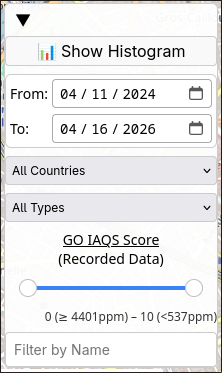
\includegraphics[width=.70\textwidth]{img/indoorco2map-filters}

\footnotesize \textit{Poznámka:} Od shora dolů: Zobrazení histogramu momentálního filtru (včetně hranice náhledu), filtrování dle časového rozsahu, filtrování dle země, filtrování dle typu lokality (restarace, škola, apod.), filtrování dle koncentrace CO\textsubscript{2} (GO IAQS skóre), filtrování podle názvu měření. 

\footnotesize \textit{Zdroj:} Snímek obrazovky pořízen autorem z webového rozhraní aplikace \parencite{IndoorCO2Atlas}.
\end{figure}

\begin{figure}[htbp!]\centering
\caption{Histogram distribuce CO\textsubscript{2} filtrované oblasti v aplikaci IndoorCO2Map}
\label{obr:indoorco2map-filters-histogram}
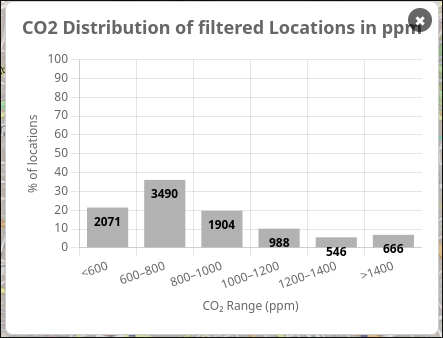
\includegraphics[width=.70\textwidth]{img/indoorco2map-filters-histogram}

\footnotesize \textit{Poznámka:} Histogram zobrazuje distribuci lokací v aktuálním filtru podle jejich průměrné koncentrace CO\textsubscript{2} v ppm.

\footnotesize \textit{Zdroj:} Snímek obrazovky pořízen autorem z webového rozhraní aplikace \parencite{IndoorCO2Atlas}.
\end{figure}

\begin{figure}[htbp!]\centering
\caption{Menu se zájmovými metrikami v aplikaci IndoorCO2Map}
\label{obr:indoorco2map-menu}
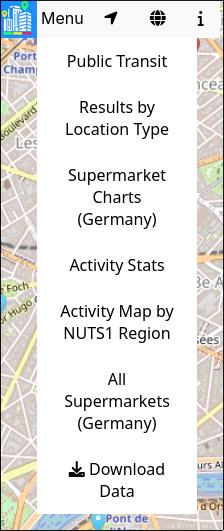
\includegraphics[width=.50\textwidth]{img/indoorco2map-menu}

\footnotesize \textit{Poznámka:} Metriky od shora: 1 - Metriky z prostorů veřejné dopravy, 2 - statistika měření pro každý typ lokace (restaurace, škola, apod.), 3 - statistika měření pro německé supermarkety, 4 - statistika aktivity měření, 5 - statistika aktivity měření podle NUTS1 regionu, 6 - zobrazní všech německých supermarketů na mapě včetně těch, které žádné měření neposkytnuly, 7 - stažení dat aktuálního náhledu 

\footnotesize \textit{Zdroj:} Snímek obrazovky pořízen autorem z webového rozhraní aplikace \parencite{IndoorCO2Atlas}.
\end{figure}


V tabulce č.~\ref{tab:indoorco2map-supported-sensors} je uveden přehled senzorů podporovaných aplikací \textit{IndoorCO2Map} a veličin, které tyto senzory hardwarově měří. Aplikace podporuje přesně čtyři modely CO\textsubscript{2} monitorů komunikujících přes rozhraní Bluetooth Low Energy (BLE); uživatel nemůže přidat vlastní typ senzoru \parencite{aurelwuAurelWuIndoorCO2MapApp2026}.

\begin{table}[!tbp]
  \centering
  \footnotesize
  \setlength{\tabcolsep}{2pt}
  \renewcommand{\arraystretch}{1.1}
  \caption{Podporované senzory IndoorCO2Map a jejich měřené veličiny relevantní pro IEQ}
  \label{tab:indoorco2map-supported-sensors}
  \begin{tabular}{l@{\hspace{12pt}}*{8}{c}@{\hspace{12pt}}*{3}{c}@{\hspace{12pt}}*{2}{c}@{\hspace{12pt}}*{2}{c}}
    \toprule
    \multirow{3}{*}{\textbf{Senzor}} & \multicolumn{15}{c}{\textbf{Kategorie IEQ}} \\
                                     & \multicolumn{8}{c}{\textbf{IAQ}} & \multicolumn{3}{c}{\textbf{TK}} & \multicolumn{2}{c}{\textbf{SK}} & \multicolumn{2}{c}{\textbf{AK}} \\
                                     & PM\textsubscript{2.5} & PM\textsubscript{10} & O\textsubscript{3} & NO\textsubscript{2} & SO\textsubscript{2} & CO & CO\textsubscript{2} & TVOC & $T$ & RH & $v$ & $E$ & CCT & $L_A$ & $L$ \\
                                     \hline
Aranet4 &  &  &  &  &  &  & \cmark &  & \cmark & \cmark &  &  &  &  &  \\
\hline
Airvalent &  &  &  &  &  &  & \cmark &  & \cmark & \cmark &  &  &  &  &  \\
\hline
AirSpot Health &  &  &  &  &  &  & \cmark &  & \cmark & \cmark &  &  &  &  &  \\
\hline
Inkbird IAM-T1 &  &  &  &  &  &  & \cmark &  & \cmark & \cmark &  &  &  &  &  \\
    \bottomrule
  \end{tabular}

  \footnotesize \textit{Zdroj:} Vlastní zpracování na základě \parencite{Aranet4HOMEIndoor, PremiumBlackAirvalent, AirSpot, INKBIRDWireless4in1}.
\end{table}

Všechny podporované senzory jsou dedikované CO\textsubscript{2} monitory využívající měřicí princip nedisperzní infračervené absorpce (NDIR) a vedle koncentrace CO\textsubscript{2} měří rovněž teplotu a relativní vlhkost \parencite{Aranet4HOMEIndoor, PremiumBlackAirvalent, AirSpot, INKBIRDWireless4in1}. Aplikace \textit{IndoorCO2Map} však z~těchto senzorů extrahuje a odesílá na backend výhradně hodnoty CO\textsubscript{2}; teplota ani vlhkost nejsou přenášeny \parencite{aurelwuAurelWuIndoorCO2MapApp2026}. Pro každý senzor existuje ve zdrojovém kódu aplikace samostatná implementace, což znamená, že aplikace je přímo závislá na konkrétním hardwaru \parencite{aurelwuAurelWuIndoorCO2MapApp2026}.

Tento přístup se zásadně odlišuje od ostatních analyzovaných aplikací. Zatímco u aplikací Sensor.Community a openSenseMap uživatel připojuje senzor k mikrokontroléru a buduje senzorovou stanici, u \textit{IndoorCO2Map} uživatel používá komerční CO\textsubscript{2} monitor spárovaný přes BLE s mobilním telefonem. Lokalizace měřeného místa rovněž nevychází přímo od uživatele — aplikace využívá OSM Overpass API k vyhledání nejbližších budov v okolí a uživatel vybírá z nabízených OSM objektů \parencite{aurelwuAurelWuIndoorCO2MapApp2026, IndoorCO2MapCO2Monitoring2024}.

Z hlediska technické architektury je mobilní aplikace multiplatformní (Android, iOS). Sběr dat probíhá v řetězci: BLE senzor odesílá data do mobilního telefonu, který je následně přenáší prostřednictvím HTTPS POST požadavku ve formátu JSON na AWS API Gateway. Backend je postaven na serverless architektuře AWS; konkrétní databáze není veřejně dokumentována. Webový frontend je implementován jako statické HTML s JavaScriptem. Aplikace podporuje dva režimy měření: měření v budově (\textit{Building}) a měření ve veřejné dopravě (\textit{Transit}) \parencite{aurelwuAurelWuIndoorCO2MapApp2026}.


\subsection{Srovnání aplikací}

V~předchozích sekcích byly jednotlivé aplikace představeny z~hlediska sbíraných dat, technického řešení, webového rozhraní a~podporovaných zařízení. Tato sekce je navzájem porovnává za účelem identifikace společných vzorů, odlišností a~mezer. Znalost těchto rozdílů je klíčová pro formulaci požadavků na vlastní aplikaci, která je cílem této práce. Srovnání vychází ze dvou souhrnných tabulek --- tabulky~\ref{tab:aplikace-srovnani-data}, která porovnává pokrytí veličin relevantních pro IEQ, a~tabulky~\ref{tab:aplikace-srovnani-technicke}, která shrnuje technické parametry. Kromě těchto tabulek sekce dále porovnává webová rozhraní a~přístupy k~hardwarové podpoře, které jsou popsány v~předchozích sekcích jednotlivých aplikací.

\begin{table}[!tbp]
  \centering
  \footnotesize
  \setlength{\tabcolsep}{2pt}
  \renewcommand{\arraystretch}{1.1}
  \caption{Srovnání vybraných aplikací dle sbíraných dat}
  \label{tab:aplikace-srovnani-data}
  \begin{tabular}{{l}@{\hspace{12pt}}{l}@{\hspace{14pt}}cccc}
    \toprule
    \multirow{2}{*}{\textbf{Kategorie IEQ}} & \multirow{2}{*}{\textbf{Veličina}} & \multicolumn{4}{c}{\textbf{Aplikace}}  \\
                               &                     & Sensor.Community & OpenAQ & OpenSense\textsuperscript{*} & IndoorCO2Map                 \\
    \hline
    \multirow{7}{*}{IAQ}               & PM\textsubscript{2.5}               & \cmark & \cmark & \cmark &  \\
                                       & PM\textsubscript{10}                & \cmark & \cmark & \cmark &  \\
                                         & O\textsubscript{3}  & & \cmark &  &  \\
                                       & NO\textsubscript{2} & \cmark & \cmark & \cmark &  \\
                                       & SO\textsubscript{2} & & \cmark & &  \\
                                       & CO                  & & \cmark & \cmark &  \\
                                       & CO\textsubscript{2} & \cmark & \cmark & \cmark & \cmark \\
                                       & TVOC                & & & \cmark &  \\
    \hline
    \multirow{3}{*}{Tepelný komfort}   & $T$ & \cmark & \cmark & \cmark &  \\
                                       & RH & \cmark & \cmark & \cmark &  \\
                                       & $v$ & & & \cmark &  \\
    \hline
    \multirow{2}{*}{Vizuální komfort}  & $E$ & & & \cmark &  \\
                                       & CCT & & & &  \\
    \hline
    \multirow{2}{*}{Akustický komfort} & $L_A$ & \cmark & & \cmark &  \\
                                       & $L$ & & & &  \\
  \bottomrule
  \end{tabular}

  \footnotesize \textsuperscript{*}OpenSenseMap umožňuje uživatelsky definovat senzory, veličiny i jednotky; uvedené veličiny jsou orientační výběr.\\
  \footnotesize \textit{Zdroj:} Vlastní zpracování na základě dat z \parencite{Index, APIs, aurelwuAurelWuIndoorCO2MapApp2026}
\end{table}

\begin{table}[!tbp]
  \centering
  \footnotesize
  \setlength{\tabcolsep}{2pt}
  \renewcommand{\arraystretch}{1.1}
  \caption{Srovnání vybraných aplikací dle technických parametrů}
  \label{tab:aplikace-srovnani-technicke}
  \begin{tabular}{p{2.8cm}p{3.1cm}p{3.0cm}p{3.0cm}p{2.7cm}}
    \toprule
     & \textbf{Sensor.Community} & \textbf{OpenAQ} & \textbf{OpenSenseMap} & \textbf{IndoorCO2Map}\\
    \midrule
      \textbf{Komunikační model} & HTTP Push & Ingest poskytovatelem dat & HTTP Push, TTN (LoRaWAN), MQTT & HTTPS POST (BLE $\rightarrow$ app $\rightarrow$ AWS)\\
    \midrule
      \textbf{Formát API} & JSON & JSON & JSON, CSV, {GeoJSON} & Neposkytuje veřejné čtecí API\\
    \midrule
      \textbf{Formát archivu} & CSV (ZIP) & CSV (GZIP) & CSV + JSON metadata & JSON (ZIP)\\
    \midrule
      \textbf{Autentizace (čtení)} & Ne & API klíč (registrace) & Ne & Ne\\
    \midrule
      \textbf{Definice veličin} & Pevný výčet & Pevný výčet & Volně definovatelné uživatelem & Pevný výčet (pouze CO\textsubscript{2})\\
    \midrule
      \textbf{Závislost na HW} & Podporované senzory & Nezávislá na HW & Nezávislá (šablony) & Podporované senzory (4 modely)\\
    \midrule
      \textbf{Rozlišení indoor/outdoor} & Ano (filtr) & Ne (primárně outdoor) & Ano (indoor, outdoor, mobile) & Výhradně indoor\\
    \midrule
      \textbf{Úložiště} & InfluxDB & PostgreSQL + Amazon S3 & MongoDB + HTTP archiv & AWS serverless\\
    \bottomrule
  \end{tabular}

  \footnotesize \textit{Zdroj:} Vlastní zpracování na základě dat z \parencite{Index, APIs, API, zotero-item-552, OpenaqOpenaqapiv22026, aurelwuAurelWuIndoorCO2MapApp2026, zotero-item-571, IndoorCO2Atlas}
\end{table}

\subsubsection{Srovnání z~pohledu sbíraných dat}

Jak ukazuje tabulka~\ref{tab:aplikace-srovnani-data}, všechny analyzované aplikace pokrývají alespoň část kategorie kvality vnitřního ovzduší (IAQ), avšak šíře pokrytí se výrazně liší. Zatímco OpenAQ eviduje osm znečišťujících látek včetně O\textsubscript{3}, SO\textsubscript{2} a~CO, které ostatní aplikace buď nesledují, nebo sledují jen omezeně, Sensor.Community a~openSenseMap se zaměřují především na mikročástice (PM\textsubscript{2,5}, PM\textsubscript{10}) a~CO\textsubscript{2}. IndoorCO2Map představuje opačný extrém --- měří výhradně koncentraci CO\textsubscript{2}, přestože podporované senzory disponují i~měřením teploty a~relativní vlhkosti \parencite{aurelwuAurelWuIndoorCO2MapApp2026}.

Veličiny tepelného komfortu (teplota a~relativní vlhkost) jsou s~výjimkou IndoorCO2Map podporovány všemi aplikacemi a~lze je považovat za de facto standard. Rychlost proudění vzduchu, která je rovněž relevantní pro hodnocení tepelného komfortu, eviduje pouze openSenseMap. Naproti tomu vizuální a~akustický komfort zůstává v~analyzovaných aplikacích výrazně podreprezentován. Osvětlenost eviduje pouze openSenseMap, hladinu akustického tlaku pak openSenseMap a~Sensor.Community. Žádná z~aplikací nesleduje korelovanou teplotu chromatičnosti (CCT) ani ekvivalentní hladinu akustického tlaku~$L$.

Koncentrace CO\textsubscript{2} je jedinou veličinou, kterou podporují všechny čtyři aplikace, což odráží její roli jako základního indikátoru kvality vnitřního vzduchu a~větrání.

Z~tohoto srovnání plyne, že žádná z~analyzovaných aplikací nepokrývá IEQ komplexně napříč všemi čtyřmi kategoriemi. openSenseMap se tomuto cíli přibližuje nejvíce díky volně definovatelným veličinám, avšak za cenu problémů s~konzistencí dat popsaných výše. Pro návrh vlastní aplikace to naznačuje prostor pro řešení, které by pokrylo všechny kategorie IEQ se zachováním konzistentní struktury měřených dat.

\subsubsection{Srovnání technického řešení}

Z~tabulky~\ref{tab:aplikace-srovnani-technicke} vyplývá, že analyzované aplikace sdílejí společný základ v~podobě formátu JSON a~archivace dat, avšak výrazně se liší v~komunikačním modelu, v~přístupu k~definici veličin a~v~míře závislosti na konkrétním hardwaru.

Z~hlediska komunikačního modelu převažuje princip HTTP Push, kdy senzorová stanice aktivně odesílá data na server. Tento model využívají Sensor.Community, openSenseMap i~IndoorCO2Map. OpenAQ se odlišuje tím, že data zpravidla nezískává přímo od senzorů, ale prostřednictvím ingestu od poskytovatelů dat, což je přístup vhodný pro agregaci rozsáhlých externích datových zdrojů. openSenseMap navíc podporuje alternativní protokoly TTN (LoRaWAN) a~MQTT, čímž rozšiřuje spektrum možností připojení senzorů nad rámec běžného HTTP.

Všechny aplikace s~výjimkou IndoorCO2Map poskytují veřejné čtecí API ve formátu JSON. openSenseMap nabízí navíc formáty CSV a~GeoJSON. Absence veřejného čtecího API u~IndoorCO2Map představuje z~hlediska principů otevřených dat výrazné omezení --- data jsou sice dostupná prostřednictvím archivu, avšak nikoliv v~reálném čase. Archivy dat nabízejí všechny analyzované aplikace, převážně ve formátu CSV. Autentizace pro čtení dat je vyžadována pouze u~OpenAQ, která vyžaduje registraci a~API klíč.

Zásadní rozdíl mezi aplikacemi spočívá v~přístupu k~definici měřených veličin. Tři ze čtyř aplikací pracují s~pevným výčtem veličin, což zajišťuje konzistenci dat, ale omezuje flexibilitu při integraci nových typů senzorů. openSenseMap volí opačný přístup --- uživatel volně definuje názvy veličin, jednotky i~typy senzorů. Tento model je ze všech analyzovaných řešení nejflexibilnější, avšak jak bylo popsáno v~sekci věnované openSenseMap, přináší problémy s~normalizací dat, kdy stejná fyzikální veličina může být evidována pod různými názvy a~v~různých jednotkách.

Obdobné rozdělení existuje i~v~míře závislosti na hardwaru. Sensor.Community a~IndoorCO2Map vyžadují použití konkrétních podporovaných senzorů, zatímco OpenAQ a~openSenseMap nejsou na hardware přímo vázány. Pro návrh vlastní aplikace představuje toto rozhodnutí klíčový kompromis mezi snadností integrace na straně jedné a~škálovatelností na straně druhé.

Z~hlediska rozlišení vnitřního a~vnějšího prostředí, které je pro tuto práci zvlášť relevantní, pouze Sensor.Community a~openSenseMap umožňují filtrovat data podle typu prostředí. OpenAQ je primárně zaměřena na venkovní monitoring a~tuto kategorizaci nepodporuje. IndoorCO2Map je orientována výhradně na vnitřní prostředí. Pro vlastní aplikaci zaměřenou na IEQ je schopnost rozlišit typ prostředí nezbytným požadavkem, aby bylo možné data o~vnitřním prostředí oddělit od dat venkovních.

\subsubsection{Webová rozhraní}

Všechny analyzované aplikace nabízejí webové rozhraní založené na interaktivní mapě, kde jsou senzory zobrazeny jako body. Tato architektura představuje v~tomto typu aplikací osvědčený standard a~poskytuje uživatelům intuitivní způsob prohlížení dat s~geografickým kontextem.

Aplikace se však liší v~rozsahu filtrů a~analytických funkcí. Sensor.Community a~OpenAQ nabízejí filtrování především podle sledované veličiny a~typu lokality, případně poskytovatele dat. openSenseMap disponuje nejkomplexnějším filtrovacím aparátem zahrnujícím omezení podle časového období, jména stanice, skupiny, modelu senzorové stanice, typu prostředí (indoor, outdoor, mobile) i~konkrétní veličiny. IndoorCO2Map přistupuje k~filtrování odlišně --- využívá typ lokality odvozený z~tagů OpenStreetMap (např. supermarket, škola, nemocnice), což odráží její zaměření na veřejně přístupné budovy a~umožňuje srovnání kvality vzduchu napříč různými typy prostor.

Většina aplikací umožňuje zobrazit aktuální hodnoty senzorů přímo na mapě. OpenAQ a~IndoorCO2Map nabízejí navíc zobrazení historických průběhů měření v~grafické podobě. IndoorCO2Map se odlišuje také histogramem distribuce lokací podle průměrné koncentrace CO\textsubscript{2} a~souhrnými statistikami podle typu lokality a~regionu NUTS\,1. Tyto analytické pohledy přesahují rámec pouhého zobrazení dat a~umožňují uživatelům identifikovat vzory a~trendy.

Pro návrh vlastní aplikace je z~tohoto srovnání relevantní, že mapová vizualizace je osvědčeným a~očekávaným standardem. Hodnotným rozšířením jsou filtry podle typu prostředí, které z~analyzovaných aplikací nabízí pouze openSenseMap. Analytické funkce nad rámec zobrazení aktuálních hodnot, jako je vizualizace historických dat či souhrnné statistiky, představují diferenciátor, který zvyšuje užitnou hodnotu platformy.

\subsubsection{Podporovaná zařízení}

Přístup k~hardwarové podpoře představuje jednu z~nejvýraznějších diferenciací mezi analyzovanými aplikacemi. Na jednom konci spektra stojí openSenseMap, která nemá žádný fixní seznam senzorů a~umožňuje uživateli zaregistrovat libovolné zařízení s~volně definovanými veličinami. Podobně OpenAQ není závislá na konkrétních senzorech, přestože v~jejích datech lze identifikovat 27 různých instrumentů. Na druhém konci spektra stojí IndoorCO2Map, která podporuje právě čtyři modely CO\textsubscript{2} monitorů komunikujících přes rozhraní Bluetooth Low Energy.

Sensor.Community zaujímá střední pozici --- podporuje přes 30 typů senzorů, avšak pro každý z~nich vyžaduje explicitní implementaci ve firmwaru senzorové stanice. Tato závislost na konkrétním hardwaru zvyšuje konzistenci přijímaných dat, ale zároveň znamená, že podpora nového senzoru vyžaduje zásah do zdrojového kódu.

Z~hlediska pokrytí kategorií IEQ se podporovaná zařízení jednotlivých aplikací výrazně liší. Senzory aplikací Sensor.Community a~OpenAQ pokrývají primárně IAQ a~tepelný komfort. Předdefinované šablony openSenseMap zahrnují i~osvětlenost a~hluk. IndoorCO2Map je omezena na CO\textsubscript{2} monitory, přestože některé z~nich hardwarově měří i~teplotu a~vlhkost, které aplikace neextrahuje \parencite{aurelwuAurelWuIndoorCO2MapApp2026}.

Odlišný je rovněž způsob integrace senzorů. Sensor.Community a~openSenseMap předpokládají, že uživatel sestaví senzorovou stanici z~mikrokontroléru a~připojených senzorů. OpenAQ přijímá data od poskytovatelů bez nutnosti přímé integrace senzoru. IndoorCO2Map se zcela odlišuje tím, že využívá komerční CO\textsubscript{2} monitory párované přes BLE s~mobilním telefonem, který data odesílá na server \parencite{aurelwuAurelWuIndoorCO2MapApp2026}.

Pro návrh vlastní aplikace toto srovnání naznačuje, že hardwarová nezávislost zvyšuje škálovatelnost platformy, avšak měla by být doplněna o~mechanismy zajišťující konzistenci dat, například prostřednictvím standardizovaného výčtu podporovaných veličin s~možností jeho budoucího rozšíření.

\subsubsection{Shrnutí srovnání}

Provedené srovnání ukazuje, že analyzované aplikace se soustředí primárně na kvalitu vnějšího ovzduší a~žádná z~nich nepokrývá oblast IEQ v~plné šíři všech čtyř kategorií --- kvality vnitřního ovzduší, tepelného, vizuálního a~akustického komfortu. Tepelný komfort a~základní ukazatele IAQ (zejména PM\textsubscript{2,5}, PM\textsubscript{10} a~CO\textsubscript{2}) jsou zastoupeny téměř univerzálně, zatímco vizuální a~akustický komfort představují výraznou mezeru.

Z~technického hlediska lze identifikovat dva dominantní přístupy: uzavřený model s~pevným výčtem veličin a~seznamem podporovaných senzorů (Sensor.Community, IndoorCO2Map) a~otevřený model s~volně definovatelnými parametry (openSenseMap). Uzavřený model zajišťuje konzistenci dat a~usnadňuje jejich agregaci, zatímco otevřený model nabízí maximální flexibilitu za cenu problémů s~normalizací. OpenAQ představuje specifický případ, kdy je hardwarová nezávislost kombinována s~pevným výčtem veličin.

Z~hlediska přístupu k~datům je pozitivním zjištěním, že všechny aplikace nabízejí archiv dat ke stažení. Většina rovněž poskytuje veřejné čtecí API, což umožňuje programatický přístup k~datům v~reálném čase. Webové rozhraní založené na interaktivní mapě je společným standardem, avšak analytické funkce nad rámec pouhého zobrazení dat nabízí pouze část aplikací.

Pro návrh vlastní aplikace z~těchto zjištění vyplývá několik klíčových směrů: pokrytí všech kategorií IEQ, rozlišení vnitřního a~vnějšího prostředí, poskytnutí veřejného čtecího API a~pravidelného archivu dat a~nalezení rovnováhy mezi flexibilitou a~konzistencí při definici veličin a~podpoře hardwaru. Tato zjištění budou vstupem pro kapitolu věnovanou analýze požadavků.


%tag-zarizeni
